\documentclass{beamer}

% There are many different themes available for Beamer. A comprehensive
% list with examples is given here:
% http://deic.uab.es/~iblanes/beamer_gallery/index_by_theme.html
% You can uncomment the themes below if you would like to use a different
% one:
%\usetheme{AnnArbor}
%\usetheme{Antibes}
%\usetheme{Bergen}
%\usetheme{Berkeley}
%\usetheme{Berlin}
%\usetheme{Boadilla}
%\usetheme{boxes}
%\usetheme{CambridgeUS}
%\usetheme{Copenhagen}
%\usetheme{Darmstadt}
%\usetheme{default}
%\usetheme{Frankfurt}
%\usetheme{Goettingen}
%\usetheme{Hannover}
%\usetheme{Ilmenau}
%\usetheme{JuanLesPins}
%\usetheme{Luebeck}
%\usetheme{Madrid}
%\usetheme{Malmoe}
%\usetheme{Marburg}
%\usetheme{Montpellier}
%\usetheme{PaloAlto}
%\usetheme{Pittsburgh}
%\usetheme{Rochester}
%\usetheme{Singapore}
%\usetheme{Szeged}
\usetheme{Warsaw}
%\usetheme{CambridgeUS}
%\usecolortheme{dolphin}
\usecolortheme{whale}

\title{Bodhitree}

\subtitle{E-learning platform development}

\author{Avijeet Gaikwad \\ 143050101}

\institute[] % (optional, but mostly needed)
{  Guided by \\
	\vspace{0.1cm}
	{\small Prof. Kameswari Chebrolu} \\
	and \\
	{\small Prof. Bhaskaran Raman} \\
	\vspace{0.5cm}
	Department of Computer Science and Engineering\\
  IIT Bombay}

\date{October 21, 2015}

\begin{document}

\begingroup
%\setbeamertemplate{headline}{}
\begin{frame}[plain]
  \titlepage
\end{frame}
\endgroup

\begin{frame}{Outline}
  \tableofcontents
  % You might wish to add the option [pausesections]
\end{frame}

% Section and subsections will appear in the presentation overview
% and table of contents.
\section[]{Bodhitree Introduction}

\subsection*{Bodhitree Introduction}

\begin{frame}{Bodhitree Introduction}{Components of the platform and introduction}
  \begin{itemize}
  \item {
    Small Private Online Courses (SPOCs)
  }
  \item {
    Bodhitree is an e-learning platform used to host SPOCs
  }
  \item {
  	Components of Bodhitree:
  	\begin{itemize}
  		\item Courseware
  		\begin{itemize}
  			\item Concepts
  			\item Discussion Forums
  			\item Assignments
  		\end{itemize}
  		\item Documents
  		\item Videos
  		\item Quizzes
  		\item ...
  	\end{itemize}
  }
  \end{itemize}
\end{frame}

\subsection*{Terminology}

\begin{frame}{Terminology}
	\begin{figure}
		\centering
		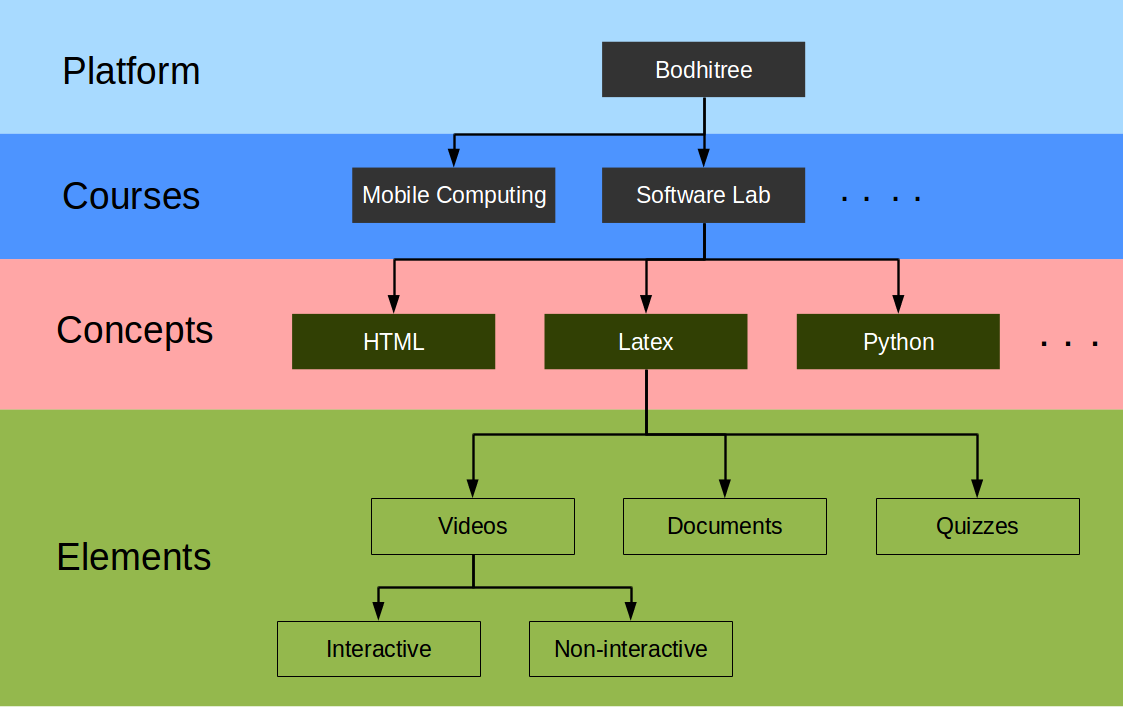
\includegraphics[width=0.8\linewidth]{media/bt}
		\caption{Components of Bodhitree and terminology}
		\label{fig:bt}
	\end{figure}

\end{frame}

\section{Marks Module}

\subsection{Problem Statement}

\begin{frame}{Marks module}{Store and display students marks}
\begin{block}{Problem Statement}
	\begin{itemize}
		\item Store student’s marks on Bodhitree
		\item Enable the students to view their marks on the course page
	\end{itemize}
\end{block}
\end{frame}

\subsection{Specifications}

\begin{frame}{Specifications}
	\begin{itemize}
		\item The instructor can upload a CSV file containing the marks of the students
		\item Student can log into his Bodhitree account and can see his marks on the course page
	\end{itemize}
\end{frame}

\begin{frame}
	Required format of the CSV file: \\
	\vspace{0.4cm}
%	\begin{itemize}
%		\item First line is the names of exams
%		\item Second line is the maximum marks of that exam
%		\item The lines that follow are the usernames of students followed by their marks
%	\end{itemize}
\centering
\begin{tabular}{|c|c|c|c|c|}
	\hline \rule[-2ex]{0pt}{5.5ex} EXAM\_TYPE & Q1 & Midsem & Q2 & Endsem \\ 
	\hline \rule[-2ex]{0pt}{5.5ex} MAX\_MARKS & 20 & 30 & 20 & 30 \\ 
	\hline \rule[-2ex]{0pt}{5.5ex} Student 1 & 18 & 25 & 12 & 22 \\ 
	\hline \rule[-2ex]{0pt}{5.5ex} Student 2 & 12 & 20 & 14 & 24 \\ 
	\hline \rule[-2ex]{0pt}{5.5ex} Student 3 & 16 & 24 & 0 & 22 \\ 
	\hline 
\end{tabular} 
\end{frame}

\subsection{Design}

\begin{frame}{Design}
	\begin{itemize}
		\item CSV file upload and storing the marks
		\item Displaying marks to the user
		\item Handling authorization
	\end{itemize}
\end{frame}

\begin{frame}{Snapshot of the tables involved in the marks module}
	\begin{figure}
	\centering
	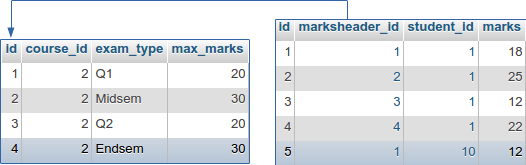
\includegraphics[width=0.8\linewidth]{media/marksdb}
	\caption{Database schema of the marks module}
	\label{fig:marksdb}
	\end{figure}

\end{frame}

\begin{frame}{Instructor's view}
	\begin{figure}
	\centering
	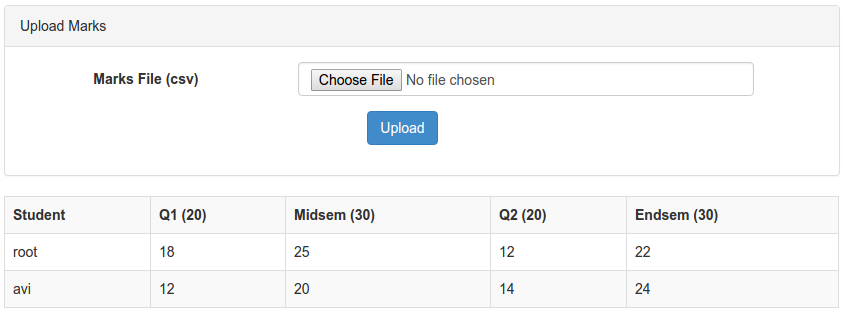
\includegraphics[width=0.8\linewidth]{media/marksi}
	\caption{Instructor's view of CSV upload and display of students marks}
	\label{fig:marksi}
	\end{figure}
\end{frame}

\begin{frame}{Student's view}
	\begin{figure}
		\centering
		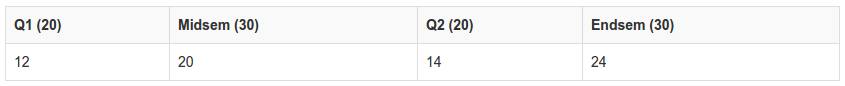
\includegraphics[width=0.8\linewidth]{media/markss1}
		\caption{Student 2's view of his marks}
		\label{fig:markss1}
	\end{figure}
\end{frame}

\section{Multimedia Textbook}

\subsection{Motivation}

\begin{frame}{Multimedia Textbook}
	\begin{figure}
		\centering
		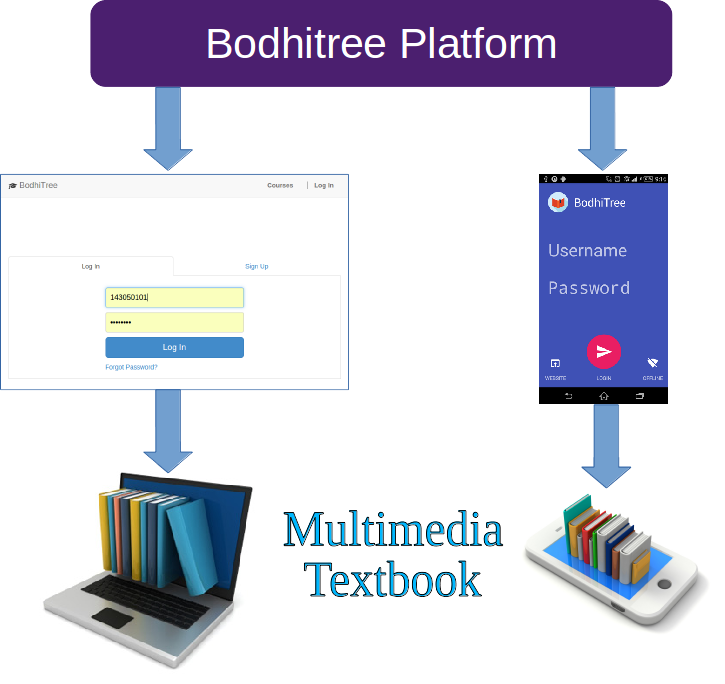
\includegraphics[width=0.6\linewidth]{media/bmmt}
		\label{fig:bmmt}
	\end{figure}
\end{frame}

\subsection{Features}

\begin{frame}{Additional Features}
	\begin{itemize}
		\item \textbf{Access Control} %Users have different privileges to the content based on payment mode
		\item \textbf{Prerequisites Graph} %A suggested dependency/schedule map of the content that shows prerequisites to content
		\item Discussion section %Clarifying doubts with peers as well as instructor
		\item Student Progress Tracking
		\item Miscellaneous:
		\begin{itemize}
			\item Accounts misuse
			\item Server and client side logging
			\item Scalability
		\end{itemize}
	\end{itemize}
\end{frame}

\section{Access Control}

\subsection{Problem Statement}

\begin{frame}{Access Control}{Differential access to content based on payment}
	\begin{block}{Problem Statement}
		\begin{itemize}
			\item 
		\end{itemize}
	\end{block}
\end{frame}

\subsection{Specifications}

\begin{frame}
	asd
\end{frame}

\subsection{System Design}

\begin{frame}
	asd
\end{frame}

\subsection{Problem statement}

\section{Prerequisite Graph}

\subsection{Problem Statement and Specifications}

\begin{frame}
	asd
\end{frame}

\subsection{System Design}

\begin{frame}
	asd
\end{frame}

\subsection{Future Work}

\begin{frame}
	asd
\end{frame}

\section*{Summary}

\end{document}